\Cref{sec:photon_selection} introduced the best-photon candidate strategy, 
as well as selection to suppress events 
where the photon is misidentified or originates in sources different than \BtoXsgamma.
However, as was seen before in, for example. \Cref{fig:photon_reco_candidates_bplus,fig:photon_reco_candidates_bzero},
\epem\ra\qqbar events provide the vast majority of photon candidates.
Therefore, a dedicated event-selection for this type of background was devised.
It takes advantage of  different event topologies expected for $\FourS\to\qqbar$ and $\epem\ra\qqbar$ events.
Loosely speaking, events where a $\FourS\to\BB$ decay is present tend to be more `spherical', when compared with $\epem\ra\qqbar$ events that exhibit a `jet-like' distribution.
This is related to the fact that \epem collissions at $B$ dactory experiments have just enough energy to produce a $B$ pair almost at rest, which means that its decays products, on average, tend to be distributed uniformly in polar and azimuthal angle.
On the other hand, light-quark pairs, produced in \epem collision events, also gain a substantial amount of back-to-back momentum which tends to spread their decay products. 
The schematic idea of this is shown in \Cref{fig:continuum_schematic}.
This section will provide an in-depth discussion on how the discrimination between \BtoXsgamma and continuum is achieved using a \BDT.

\begin{figure}[htbp!]
    \centering
    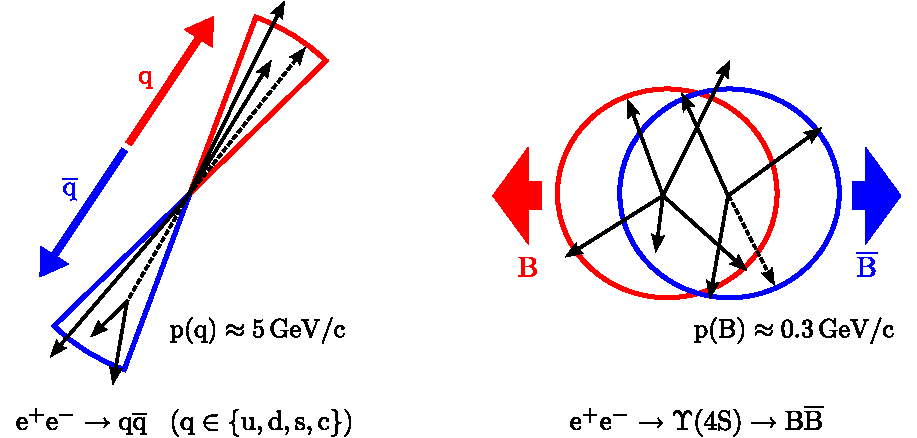
\includegraphics[width=0.6\textwidth]{figures/continuum_suppression/figure_continuum_suppression_event_shapes.pdf}
    \caption{\label{fig:continuum_schematic} Schematic illustration of continuum and \BB events created after an \epem collision in $B$ factories.
    Events where a $B$ meson is produced are generally more spherical, due to the fact that \FourS is produced at rest and its decays products tend to not have a preferred direction.
    Typical momenta of light-quark and \BB mesons are shown.
    The specific directions shown are illustrative only. 
    }
\end{figure}

\subsection{Training event pre-selection}\label{sec:preselection}

Before a \BDT is trained, it is generally desirable to prepare the datasets such that the classifier 
is able to learn based on relevant data.
Such data preprocessing will be performed based on variables described in \Cref{sec:photon_selection}.
The classifier will then be trained on the reduced dataset

In order to find optimal selections, a figure-of-merit study is performed for each observable.
Two figure of merit options were considered for this analysis, a more standard figure-of-merit $\mathrm{FOM}_1$:
\begin{equation}\label{eq:soversqrtsplusb}
    \mathrm{FOM}_1 = \frac{S}{\sqrt{S+B}},
\end{equation}
and $\mathrm{FOM}_2$ defined in Ref.\cite{Punzi:2003bu}, (sometimes referred to as `Punzi' figure-of-merit):
\begin{equation}\label{eq:punzi_fom}
    \mathrm{FOM}_2 = \frac{S}{S_0} \frac{1}{\frac{3}{2}+\sqrt{B}}.
\end{equation}
In both equations, $S$ is the number of signal events after selection, 
$B$ is the number of background events after selection, 
and $S_0$ is the number of signal events before selection.

